\documentclass[11pt,compress,t,notes=noshow, xcolor=table]{beamer}
\usepackage[]{graphicx}\usepackage[]{color}
% maxwidth is the original width if it is less than linewidth
% otherwise use linewidth (to make sure the graphics do not exceed the margin)
\makeatletter
\def\maxwidth{ %
  \ifdim\Gin@nat@width>\linewidth
    \linewidth
  \else
    \Gin@nat@width
  \fi
}
\makeatother

\definecolor{fgcolor}{rgb}{0.345, 0.345, 0.345}
\newcommand{\hlnum}[1]{\textcolor[rgb]{0.686,0.059,0.569}{#1}}%
\newcommand{\hlstr}[1]{\textcolor[rgb]{0.192,0.494,0.8}{#1}}%
\newcommand{\hlcom}[1]{\textcolor[rgb]{0.678,0.584,0.686}{\textit{#1}}}%
\newcommand{\hlopt}[1]{\textcolor[rgb]{0,0,0}{#1}}%
\newcommand{\hlstd}[1]{\textcolor[rgb]{0.345,0.345,0.345}{#1}}%
\newcommand{\hlkwa}[1]{\textcolor[rgb]{0.161,0.373,0.58}{\textbf{#1}}}%
\newcommand{\hlkwb}[1]{\textcolor[rgb]{0.69,0.353,0.396}{#1}}%
\newcommand{\hlkwc}[1]{\textcolor[rgb]{0.333,0.667,0.333}{#1}}%
\newcommand{\hlkwd}[1]{\textcolor[rgb]{0.737,0.353,0.396}{\textbf{#1}}}%
\let\hlipl\hlkwb

\usepackage{framed}
\makeatletter
\newenvironment{kframe}{%
 \def\at@end@of@kframe{}%
 \ifinner\ifhmode%
  \def\at@end@of@kframe{\end{minipage}}%
  \begin{minipage}{\columnwidth}%
 \fi\fi%
 \def\FrameCommand##1{\hskip\@totalleftmargin \hskip-\fboxsep
 \colorbox{shadecolor}{##1}\hskip-\fboxsep
     % There is no \\@totalrightmargin, so:
     \hskip-\linewidth \hskip-\@totalleftmargin \hskip\columnwidth}%
 \MakeFramed {\advance\hsize-\width
   \@totalleftmargin\z@ \linewidth\hsize
   \@setminipage}}%
 {\par\unskip\endMakeFramed%
 \at@end@of@kframe}
\makeatother

\definecolor{shadecolor}{rgb}{.97, .97, .97}
\definecolor{messagecolor}{rgb}{0, 0, 0}
\definecolor{warningcolor}{rgb}{1, 0, 1}
\definecolor{errorcolor}{rgb}{1, 0, 0}
\newenvironment{knitrout}{}{} % an empty environment to be redefined in TeX

\usepackage{alltt}
\newcommand{\SweaveOpts}[1]{}  % do not interfere with LaTeX
\newcommand{\SweaveInput}[1]{} % because they are not real TeX commands
\newcommand{\Sexpr}[1]{}       % will only be parsed by R



\usepackage[english]{babel}
\usepackage[utf8]{inputenc}

\usepackage{dsfont}
\usepackage{verbatim}
\usepackage{amsmath}
\usepackage{amsfonts}
\usepackage{bm}
\usepackage{csquotes}
\usepackage{multirow}
\usepackage{longtable}
\usepackage{booktabs}
\usepackage{enumerate}
\usepackage[absolute,overlay]{textpos}
\usepackage{psfrag}
\usepackage{algorithm}
\usepackage{algpseudocode}
\usepackage{eqnarray}
\usepackage{arydshln}
\usepackage{tabularx}
\usepackage{placeins}
\usepackage{tikz}
\usepackage{setspace}
\usepackage{colortbl}
\usepackage{mathtools}
\usepackage{wrapfig}
\usepackage{bm}
\usetikzlibrary{shapes,arrows,automata,positioning,calc,chains,trees, shadows}
\tikzset{
  %Define standard arrow tip
  >=stealth',
  %Define style for boxes
  punkt/.style={
    rectangle,
    rounded corners,
    draw=black, very thick,
    text width=6.5em,
    minimum height=2em,
    text centered},
  % Define arrow style
  pil/.style={
    ->,
    thick,
    shorten <=2pt,
    shorten >=2pt,}
}
\usepackage{subfig}


% Defines macros and environments

% basic latex stuff
\newcommand{\pkg}[1]{{\fontseries{b}\selectfont #1}} %fontstyle for R packages
\newcommand{\lz}{\vspace{0.5cm}} %vertical space
\newcommand{\dlz}{\vspace{1cm}} %double vertical space
\newcommand{\mat}[1]{ %short pmatrix command
  \begin{pmatrix}
    #1
  \end{pmatrix}
}
\newcommand{\oneliner}[1] % Oneliner for important statements
{\begin{block}{}\begin{center}\begin{Large}#1\end{Large}\end{center}\end{block}}


% 
% basic latex stuff
\newcommand{\pkg}[1]{{\fontseries{b}\selectfont #1}} %fontstyle for R packages
\newcommand{\lz}{\vspace{0.5cm}} %vertical space
\newcommand{\dlz}{\vspace{1cm}} %double vertical space
\newcommand{\mat}[1]{ %short pmatrix command
  \begin{pmatrix}
    #1
  \end{pmatrix}
}
\newcommand{\oneliner}[1] % Oneliner for important statements
{\begin{block}{}\begin{center}\begin{Large}#1\end{Large}\end{center}\end{block}}



%\usetheme{lmu-lecture}
\usepackage{../../style/lmu-lecture}

\let\code=\texttt
\let\proglang=\textsf

\setkeys{Gin}{width=0.9\textwidth}

\title{Introduction to Machine Learning}
% \author{Bernd Bischl, Christoph Molnar, Daniel Schalk, Fabian Scheipl}
\institute{\href{https://compstat-lmu.github.io/lecture_i2ml/}{compstat-lmu.github.io/lecture\_i2ml}}
\date{}

\setbeamertemplate{frametitle}{\expandafter\uppercase\expandafter\insertframetitle}



\begin{document}
% Introduction to Machine Learning
% Day 3

% Set style/preamble.Rnw as parent.


% Load all R packages and set up knitr

% This file loads R packages, configures knitr options and sets preamble.Rnw as parent file
% IF YOU MODIFY THIS, PLZ ALSO MODIFY setup.Rmd ACCORDINGLY...








%! includes: evaluation-intro

\lecturechapter{Evaluation: Overfitting}
\lecture{Introduction to Machine Learning}

\begin{vbframe}{Overfitting}

\begin{columns}[T,onlytextwidth]
\column{0.5\textwidth}
Overfitting learner \\
\vspace{0.5cm}
\begin{knitrout}\scriptsize
\definecolor{shadecolor}{rgb}{0.969, 0.969, 0.969}\color{fgcolor}

{\centering 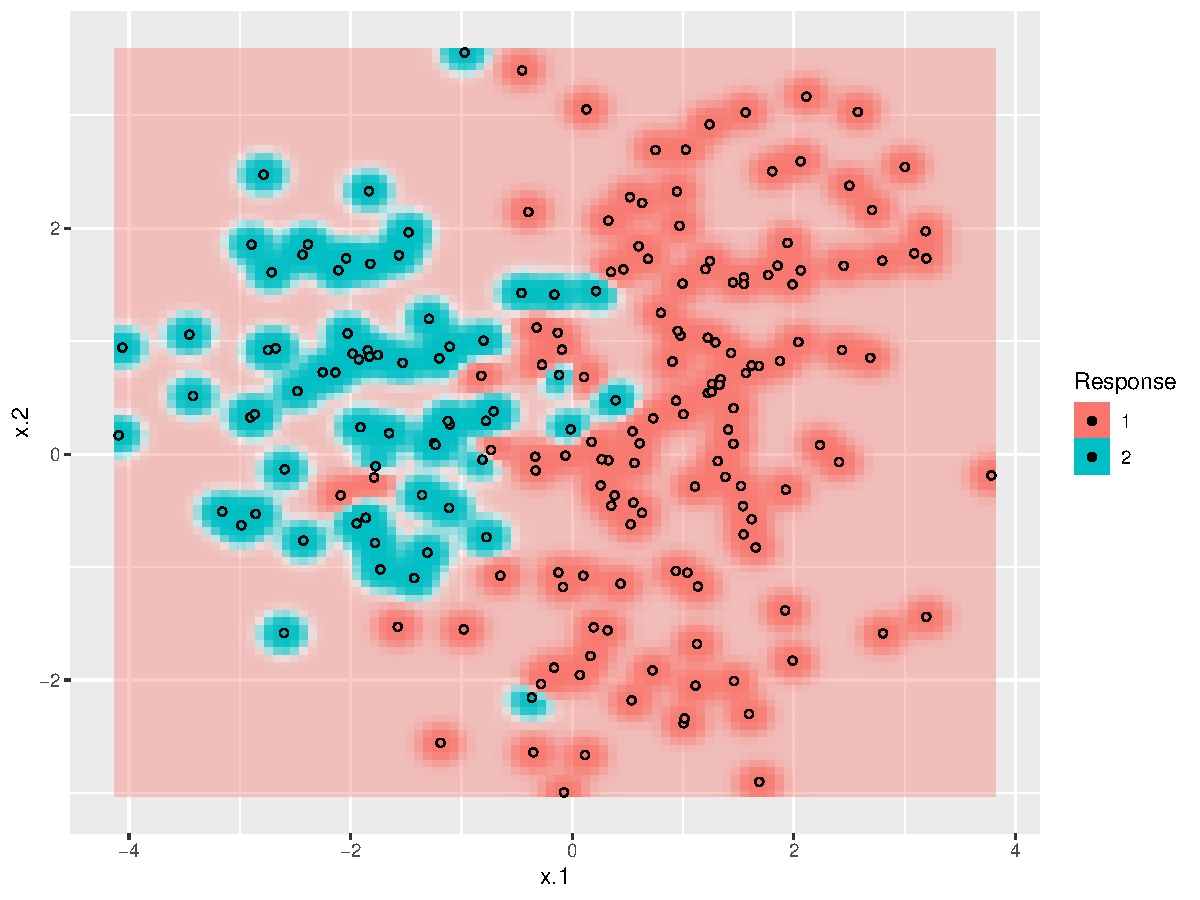
\includegraphics[width=\textwidth]{images/eval_ofit_1} 

}



\end{knitrout}
Better training set performance (seen examples)

\column{0.5\textwidth}
Non-overfitting learner \\
\vspace{0.5cm}
\begin{knitrout}\scriptsize
\definecolor{shadecolor}{rgb}{0.969, 0.969, 0.969}\color{fgcolor}

{\centering 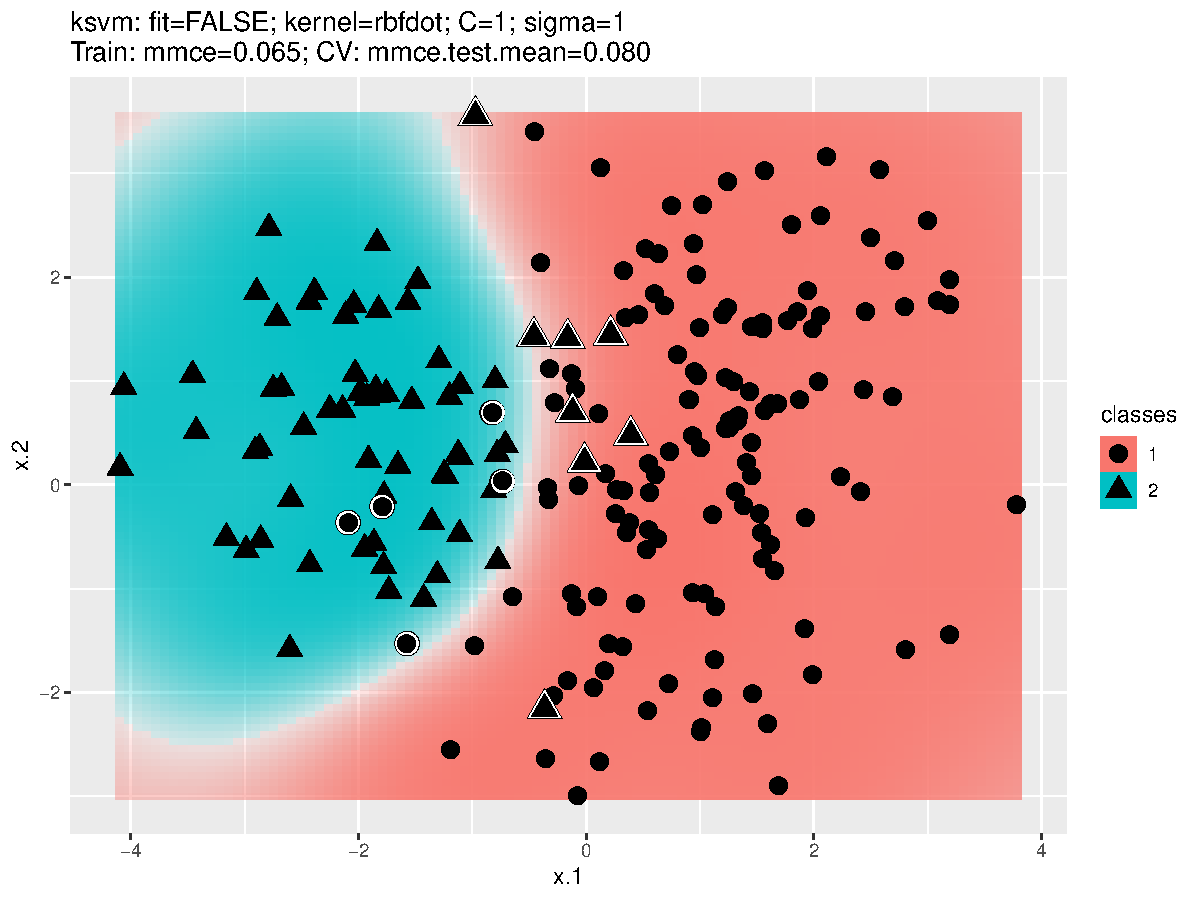
\includegraphics[width=\textwidth]{images/eval_ofit_2} 

}



\end{knitrout}
Better test set performance (unseen examples)
\end{columns}


\framebreak


\begin{itemize}
  \item Happens when algorithm models patterns beyond the data generating porcess,
    e.g., noise or artefacts in the training data
  \item Reason: Too many hypotheses and not enough data to tell them apart
  \item Less in bigger data sets
  \item If hypothesis space is not constrained, there may never be enough data
  \item Many learners have a parameter that allows constraining (\textit{regularization})
  % \item In this unit we will only give a very basic definition, and not really talk
  %   about measures against overfitting (see regularization!)
  \item Check for overfitting by validating on a new unseen test data set.
\end{itemize}

\end{vbframe}


% \begin{vbframe}{Overfitting and Noise}
% \begin{itemize}
%   \item Overfitting is seriously exacerbated by \textit{noise} (errors in the training data)
%   \item An unconstrained learner will start to model that noise
%   \item It can also arise when relevant features are missing in the data
%   \item In general it's better to make some mistakes on training data ("ignore some observations") than trying to get all correct
% \end{itemize}
% \end{vbframe}

% \begin{vbframe}{Avoiding Overfitting}
% \begin{itemize}
%   \item You should never believe your model until you've \textit{verified it on data that the learner didn't see}
%   \item Scientific method applied to machine learning: model must make new predictions that can be experimentally verified
%   \item Use less complex models 
%   \item Get more, or better data
%   \item Some learner can do "early stopping" before perfectly fitting (i.e., overfitting) the training data
%   \item Use regularization
% \end{itemize}
% \end{vbframe}

% \begin{vbframe}{Triple Trade-Off}

% In all learning algorithms that are trained from data, there is a trade-off between three factors:
% \begin{itemize}
  % \item The complexity of the hypothesis we fit to the training data
  % \item The amount of training data (in terms of both instances and informative features)
  % \item The generalization error on new examples
% \end{itemize}
% If the capacity of the learning algorithm is large enough to a) approximate the data generating process and b) exploit the information contained in the data, the generalization error will decrease as the amount of training data increases.

% For a fixed size of training data, the generalization error decreases first and then starts to increase (overfitting) as the complexity of the hypothesis space $H$ increases.
% \end{vbframe}

\begin{vbframe}{Trade-Off Between Generalization Error and Complexity}

% Apparent error (on the training data) and real error (prediction error on new data) evolve in the opposite direction with increasing complexity:

\lz
\begin{knitrout}\scriptsize
\definecolor{shadecolor}{rgb}{0.969, 0.969, 0.969}\color{fgcolor}

{\centering 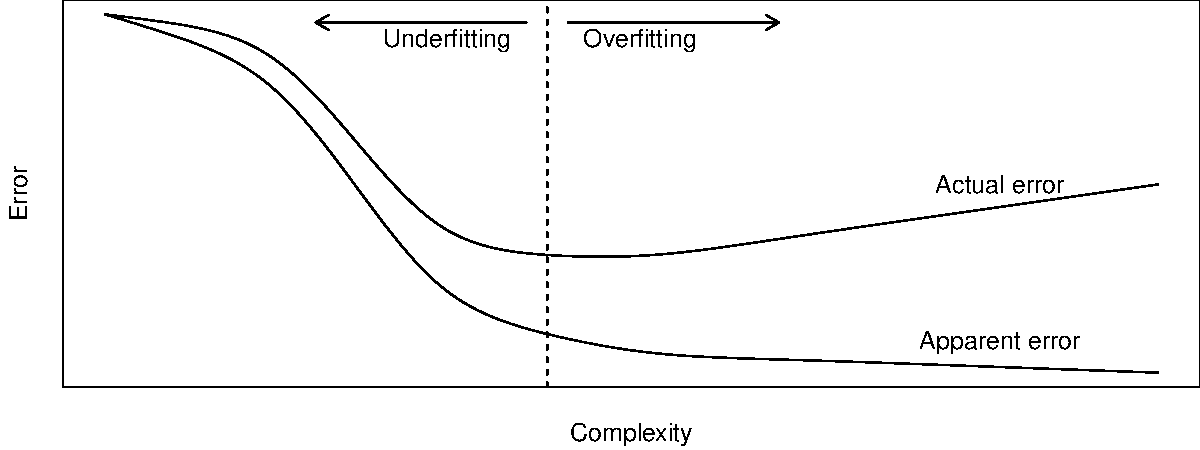
\includegraphics[width=0.95\textwidth]{images/eval_ofit_3} 

}



\end{knitrout}

\lz
$\Rightarrow$ Optimization regarding the model complexity is desirable:\\ 
Find the right amount of complexity for the given amount of data where generalization error becomes minimal.

\end{vbframe}

\endlecture
\end{document}
